 \documentclass[12pt]{article}
\usepackage[a4paper, margin=.30in]{geometry}

\usepackage{array}
\usepackage{graphicx, subfig, wrapfig, fancyhdr, lastpage }
\newcommand\headerMe[2]{\noindent{}#1\hfill#2}
\usepackage[mathscr]{euscript}



\pagestyle{fancy}
\fancyhf{}

\rfoot{\em{Page \thepage \hspace{1pt} / \pageref{LastPage}}}
\begin{document}

\headerMe{Royaume du Maroc}{année scolaire \emph{2021-2022}}\\
\headerMe{Ministère de l'Éducation nationale, }{  Professeur :\emph{Zakaria Haouzan}}\\
\headerMe{du Préscolaire et des Sports}{Établissement : \emph{Lycée SKHOR qualifiant}}\\

\begin{center}
Devoir  N°2 \\
   Filière Tronc Commun Scientifique\\
Durée 1h00
\\
    \vspace{.2cm}
\hrulefill
\Large{Chimie 7pts}
\hrulefill\\

    %\emph{Les Trois parties sont indépendantes}
\end{center}
%end Headerss------------------------
 \section*{Partie 1 :La quantité de matière \dotfill (7pts) }
La caféine, présente dans le café, le thé, le chocolat, les boissons au cola, est un stimulant pouvant être toxique à forte dose (plus de $600 mg$ par jour). Sa formule chimique est $C_8H_{10}N_4O_2$.

\begin{enumerate}
    \item Quelle est la masse molaire de la caféine?(avec M(N) = 14g/mol)\dotfill(1pt)
    \item Quelle quantité de matière de caféine y-a-t-il dans une tasse de café contenant 80 mg de caféine?\dotfill(1pt)
    \item Combien y-a-t-il de molécules de caféine dans la tasse?\dotfill(1pt)
    \item Combien de tasses de café peut-on boire par jour sans risque d’intoxication?\dotfill(2pt)
        \item Un café décaféiné en grains (ou moulu) ne doit pas contenir plus de 0,10 \% en masse de caféine.Quelle quantité de matière maximale de caféine y-a-t-il dans un paquet de café décaféiné de masse
            250g ?\dotfill(2pt)
\end{enumerate}
%__________________Chimie ______________________-
%%%%%%%+_+_+_+_+_+_+_+_+_Partie1

%_____________________________________PHYSIque Partie 22222____________________________________________________________________________
\begin{center}
    %\vspace{2cm}
\hrulefill
\Large{Physique 13pts}
\hrulefill\\
    %\emph{Les deux parties sont indépendantes}
\end{center}
%end Headerss------------------------

 \section*{Partie 1 :Le courant électrique continu \dotfill(7 pts)}

\begin{wrapfigure}[7]{r}{0.40\textwidth}
    \vspace{-1cm}
    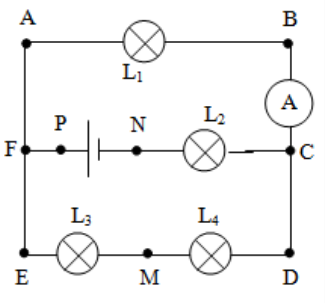
\includegraphics[width=0.36\textwidth]{./img/circuit_00.png}
\end{wrapfigure}

On considère le circuit de la figure ci-contre : 

\begin{enumerate}
    \item Sachant que la quantité d’électricité Q qui traverse la section du fil AF pendant une minute est Q = 30 C.
        \begin{enumerate}
                \item Calculer le nombre d’électrons qui traverse cette section pendant
                    la même durée.\dotfill(1pt)
                \item En déduire la valeur de l’intensité du courant $I_1$ qui traverse la lampe $L_1$ .\dotfill(1pt)
        \end{enumerate}
    \item L’ampèremètre A comporte 100 divisions et possède les calibres suivant : $5A$ ; $1 A$ ; $300 mA$ ; $100 mA$.
        \begin{enumerate}
            \item Quel est le calibre le plus adapté pour la mesure de l’intensité $I_1$?\dotfill(1pt)
            \item Devant quelle division l’aiguille de l’ampèremètre s’arrête-t-elle ?\dotfill(1pt)

        \end{enumerate}
    \item L’intensité débité par le générateur est 0,8 A.
        \begin{enumerate}
            \item Quels sont les points qui sont considérés comme des nœuds ?\dotfill(1pt)
                \item Indiquer le sens du courant dans chaque branche.\dotfill(1pt)
                \item  Déterminer les valeurs des intensités qui traversent les lampes $L_2$ , $L_3$ et $L_4$ .\dotfill(1pt)
        \end{enumerate}
\end{enumerate}

\vspace{3cm}

\hrulefill\\
%_________________partie 2  : gravitation universelle :)
\section*{Partie 2 : La Mesure de l’intensité du courant éléctrique: \dotfill(6pts)}

\begin{wrapfigure}[6]{r}{0.40\textwidth}
    \vspace{-1cm}
\begin{center}
    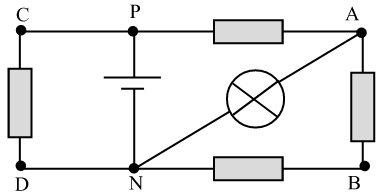
\includegraphics[width=0.36\textwidth]{./img/circuit_01.png}
\end{center}
    \end{wrapfigure}
On réalise le montage de la figure ci-contre.
\begin{enumerate}
    \item Indiquer le sens des différents courants électriques dans les
        branches du circuit.\dotfill(2pt)
    \item Compléter le tableau des intensités.\dotfill(2pt)
          \begin{tabular}{ | l | l | l | l |l|l|l|l|l|}
    \hline
              Branche       & NP & PA & AB & BN & PC & CD & DN & AN  \\\hline
              Intensité (A) & 3   &    &    & 0.5   &    &  &1       &       \\ \hline
    \end{tabular}
\item Compléter les tableaux suivants (C : Calibre ; n : nombre de division indiqué par l’aiguille ; n 0  : nombre de
    division de cadran)\dotfill(2pt)
\begin{center}
    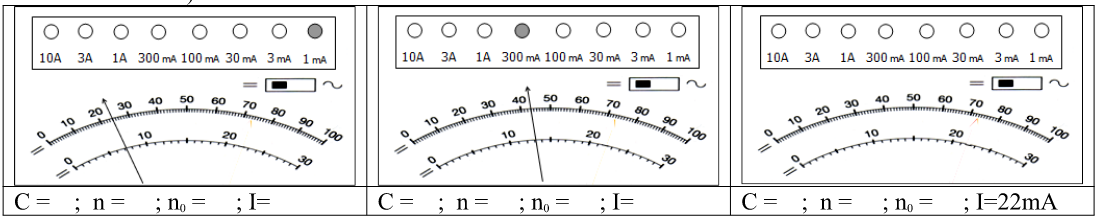
\includegraphics[width=0.95\textwidth]{./img/circuit_03.png}
\end{center}

\end{enumerate}

\end{document}
